\documentclass[a4paper,11pt,twoside,openright]{book}							% COMANDI INIZIALI
\usepackage[italian]{babel}								% sillabazione italiana
\usepackage[utf8]{inputenc}								% Per le lettere accentate IN UNIX E IN WINDOWS
\usepackage{ragged2e}					 				% giustifica
\usepackage{amsmath}									% Per allineare le equazioni
\usepackage{amssymb}									% Per le lettere dell'indicatrice (mathbb)

\usepackage{graphicx}
\usepackage{amsthm}
\usepackage{amssymb}
\usepackage{amsmath}
\usepackage{mathtools}
\usepackage{caption}
\usepackage{booktabs}
\usepackage{hyperref}
\usepackage{float}
\usepackage{subfigure}
\usepackage{multirow}
\usepackage{array}



\justifying 										% giustifica

\date{28 Luglio 2014}
\author{Gabriele Mazza}
\title{Rifiuti nella provincia di Venezia}

\begin{document}

%Indice e numerazione
\pagenumbering{arabic}

\chapter{Venezia}

Come è già stato brevemente accennato in precedenza, l'applicazione scelta per il modello STR-PDE riguarda i dati della produzione di rifiuti urbani nel periodo di anni dal 1997 al 2011 nella provincia di Venezia. Per rifiuti urbani si intendono rifiuti domestici, prodotti in locali, aree pubbliche, parchi o giardini, spiagge o provenienti dalla pulizia delle strade o di altri luoghi pubblici. Non sono conteggiati i rifiuti speciali (tra cui ad esempio gli industriali, agricoli o provenienti da attività commerciali o di costruzione) o pericolosi (per i quali esistono programmi di smaltimento particolari).

In realtà i dati raccolti dall'Agenzia Regionale per la Prevenzione e Protezione Ambientale del Veneto (Arpav) riguardano tutto il Veneto. Tuttavia è stata analizzata solo la provincia di Venezia per due motivi. Inanzitutto l'interesse particolare per la zona della laguna veneta, in cui è rilevante il ruolo del turismo (come si potrà notare in seguito). Inoltre considerare tutto il Veneto aumenta notevolmente le dimensioni delle matrici in gioco e causa una grossa spesa computazionale per la ricerca della soluzione. Quindi è stato scelto di concentrarsi su un dominio più piccolo ma nel quale è possibile notare più facilmente le particolarità dell'andamento del fenomeno della produzione dei rifiuti urbani.

Per ogni comune della provincia di Venezia e per ogni anno è disponibile il numero di rifiuti totali raccolti in tonnellate e la popolazione residente. La popolazione è certamente un valore influente per la produzione di rifiuti, perciò la quantità di riferimento non sarà il valore dei rifiuti totali raccolti in ogni anno per comune, ma il valore pro capite.

Le coordinate spaziali dei comuni sono la longitudine e la latitudine, disponibili on line\footnote{\href{http://www.dossier.net/utilities/coordinate-geografiche/}{http://www.dossier.net/utilities/coordinate-geografiche/}}. Nel caso dei comuni con dato replicato (sez \ref{sez:comunireplicati}), sono state scaricate da Google Maps.


\section{L'inclusione dell'effetto del turismo}

L'inclusione della popolazione residente nella risposta tramite la scelta di usare i valori pro capite è necessaria, poichè permette di depurare la risposta da una variabile che per sua natura la influenzerebbe. Ma sarebbe un errore fermarsi solo alla popolazione residente, poichè anche i turisti rappresentano una componente non trascurabile di produzione di rifiuti urbani.

Nella provincia di Venezia sono presenti molte zone di elevata attrazione turistica. La più rilevante di queste è Venezia, ma si hanno anche zone balneari (come Lido di Venezia, Cavallino-Treporti, Jesolo, San Michele al Tagliamento, Bibione, ecc...). L'informazione scelta per sintetizzare l'attività turistica è il numero di posti letto totali del comune, valore disponibile grazie all'applicativo dell'Istat \textit{Atlante Statistico dei Comuni}\footnote{\href{http://www.istat.it/it/archivio/113712}{http://www.istat.it/it/archivio/113712}} per ogni anno. Il totale dei posti letto per comune è la somma di vari tipi di attività non solamente alberghiere (ad esempio sono conteggiati anche esercizi complementari, bed \& breakfast, campeggi) e saranno considerati normalizzati per la popolazione residente per uniformità con la risposta. I valori ricavati saranno inseriti nel modello come possibile covariata.


\section{Trattamento del dominio}

Per poter studiare il problema a livello computazionale occorre avere una buona approssimazione della frontiera della regione. Questa è disponibile nel pacchetto R \textit{raster} che descrive dati geografici di moltissime zone del mondo sia a livello nazionale che locale (nel caso italiano province e comuni) tramite poligoni molto precisi.

Una volta scaricata la provincia di Venezia si è riscontrato subito un problema: la regione è composta da un insieme di 101 poligoni distinti (a causa delle numerose isole di cui è composta la laguna di Venezia) e ogni poligono ha un alto numero di vertici (ad esempio, la prima delle due regioni corrispondenti all'entroterra aveva 10538 vertici). Non è possibile analizzare il problema su un territorio così descritto, perciò è stata necessaria una analisi iniziale della frontiera per ridurne la complessità.

Oltre all'entroterra (composto da due poligoni) stati scelte solo le più importanti isole della laguna veneta: Venezia, Murano, Lido di Venezia e Pellestrina (più rilevanti a livello di popolazione e turismo). I poligoni sono stati semplificati in tutti i casi e uniti tra loro con ponti dove era possibile. Tra le isole collegate solamente via mare con il resto del territorio sono state simulati ponti in corrispondenza delle trafficate linee di trasporto pubblico con traghetto.

\subsection{Regression splines}

Per ridurre l'elevato numero di vertici di ognuno dei poligoni considerati si è scelto di ricorrere ad un'analisi di smoothing di dati funzionali. Ad ogni poligono è associata una coppia di funzioni: la latitudine e la longitudine rispetto all'ascissa curvilinea (disponibili per punti, corrispondenti ai vertici) che sono state rappresentate in basi e valutate in un mumero molto inferiore di punti, con i quali si è costruita la nuova definizione della regione.

Per avere una rappresentazione tramite funzioni di base di queste funzioni sono state provate più tecniche, ma la scelta definitiva è ricaduta sulle \textit{Regression Splines} cubiche senza penalizzazione della derivata seconda. Infatti i risultati non sono stati migliori negli altri casi a causa della zona interna alla laguna di Venezia, fortemente frastagliata: penalizzare la derivata seconda eliminava troppe asperità presenti sulle coste del territorio, mentre con \textit{Kernel Smoothing} sono state ricavate regioni che, dopo la triangolazione, presentavano troppi triangoli composti solamente da punti di frontiera (e quindi senza dati) rispetto agli altri metodi.

Una volta fissato un ragionevole numero di punti con cui descrivere la regione sono stati eseguiti più tentativi per decidere il miglior numero di basi necessario per descrivere le due funzioni. Il criterio di scelta è stato complesso, poichè sono stati esclusi i valori che generavano intersezioni nella nuova descrizione della regione e comuni esterni alla frontiera. Ma la scelta del miglior numero di basi per \textit{Regression Splines} è ricaduta sul valore che, una volta eseguito lo smoothing della regione, causava la minor distanza tra i nuovi punti della regione e il poligono iniziale. In figura \ref{fig:Ven_ent1} è riportato il risultato dello smoothing sul primo poligono che descrive l'entroterra della provincia di Venezia (descritta con 100 punti, molto meno dei 10538 iniziali).  

\begin{figure}[!t]
\centering
\begin{minipage}{.32\textwidth}
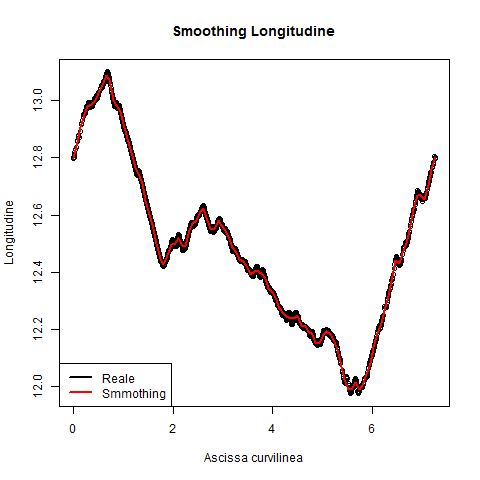
\includegraphics[width=\textwidth]{Immagini/Ven_Longitudine.png}
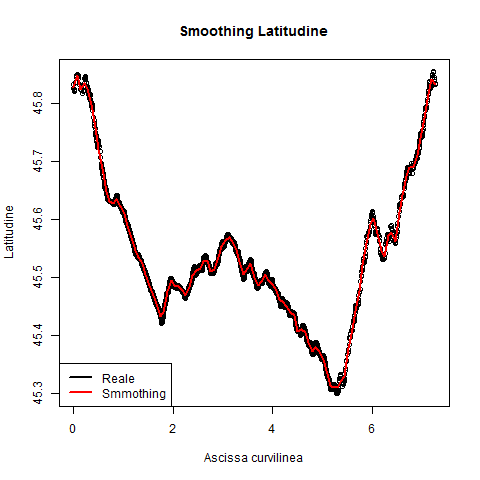
\includegraphics[width=\textwidth]{Immagini/Ven_Latitudine.png}
\end{minipage}%
\begin{minipage}{.64\textwidth}
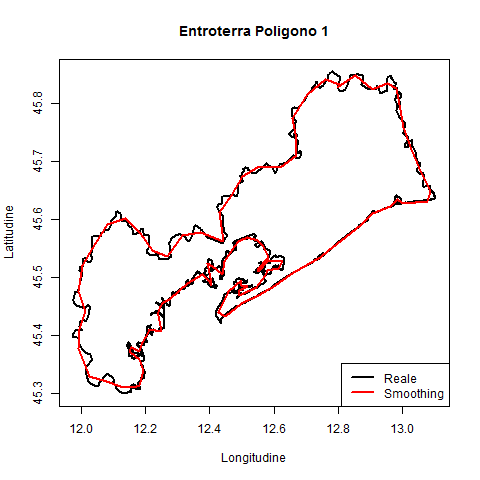
\includegraphics[width=\textwidth]{Immagini/Ven_Regione.png}
\end{minipage}
\caption{Smoothing con \textit{Regression Splines} cubiche per il primo poligono dell'entroterra della provincia di Venezia}
\label{fig:Ven_ent1}
\end{figure}

Dopo aver ripetuto l'analisi per ognuna delle isole scelte inizialmente la descrizione finale è stata ricavata unendo tra loro tutti i nuovi poligoni. In seguito è stata eliminata una zona costiera dell'entroterra della laguna di Venezia che, sebbene sia presente sia in \textit{raster} che nei grafici di Google Maps, corrisponde ad una parte fangosa e paludosa e quindi disabitata. Non essendo possibile che su di essa siano prodotti rifiuti è stata tagliata dalla regione. Per questo motivo si troverà sempre una zona non analizzata sui grafici con mappe da Google Maps. In figura \ref{fig:Ven_rgm} è riportata la descrizione finale del dominio con i punti spaziali considerati (si consulti anche la sezione \ref{sez:comunireplicati}).
\begin{figure}[t]
\centering
\subfigure[Provincia di Venezia]
   {
   \label{fig:Ven_rgm_tot}
	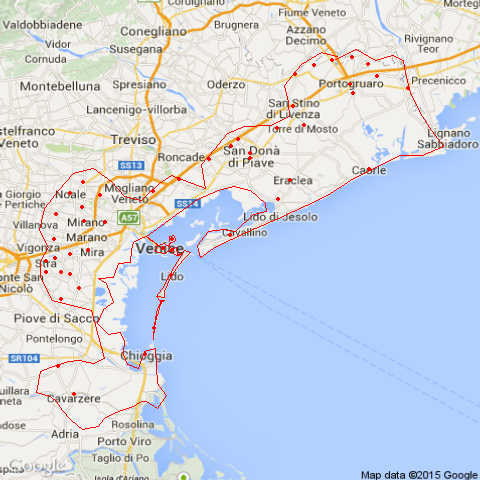
\includegraphics[width=0.46\textwidth]{Immagini/Ven_punti.png}   
   }
\subfigure[Zoom della laguna]
   {
   \label{fig:Ven_rgm_zoom}
	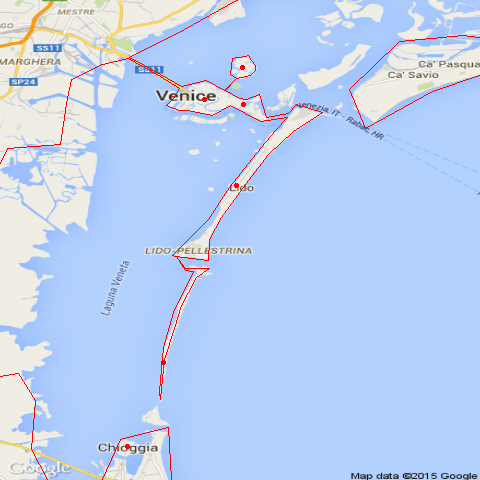
\includegraphics[width=0.46\textwidth]{Immagini/Ven_puntizoom.png}
   }
\caption{Frontiera e punti spaziali per la provincia di Venezia}
\label{fig:Ven_rgm}
\end{figure}

\subsection{Scelte particolari tra i comuni}
\label{sez:comunireplicati}

L'uso di valori pro capite per rifiuti e posti letto consente di replicare del comune anche su altri punti in cui risulta necessario. Ad esempio, le isole di Murano, Lido di Venezia e Pellestrina non sono sedi di comune, ma si riferiscono a Venezia. Quindi il dato di Venezia è stato replicato in queste isole ad ogni anno, per avere un valore di riferimento in quanto zone distaccate. Come si può notare in figura \ref{fig:Ven_rgm_zoom} anche nell'isola di Venezia è stato duplicato il dato, per avere una triangolazione  senza troppi triangoli composti solo da punti di frontiera in una zona della provincia di Venezia di particolare rilevanza.

Un caso particolare riguarda il comune di Cavallino-Treporti, che è stato istituito nel 1999 da una parte dei territori del comune di Venezia. La separazione all'interno dei dati, però, è presente dal 2002. Di conseguenza prima di questo anno il dato in Cavallino-Treporti è una replica del dato di Venezia.

\subsection{Triangolazione del dominio}

La triangolazione è stata prodotta tramite il pacchetto R \textit{RTriangle}. Poichè nella zona ad est il numero di capoluoghi di comune (e quindi di nodi della triangolazione) è minore rispetto al resto della regione, è stata fissata un'area massima per i triangoli generati da \textit{RTriangle}. Questo ha reso la triangolazione più fitta anche dove non lo sarebbe stata, e garantirà una stima della risposta più precisa nella zona balneare ad est, che come si potrà notare in seguito ha una grande importanza per la distribuzione dei rifiuti. Affinchè questo sia possibile sono stati aggiuhnti nuovi punti spaziali, che restano senza dato per tutta l'analisi. In fig. \ref{fig:Ven_triang} si ha la triangolazione finale cje sarà usata da ora in avanti.

\begin{figure}[!t]
\centering
\subfigure[Provincia di Venezia]
   {
   \label{fig:Ven_triang_tot}
	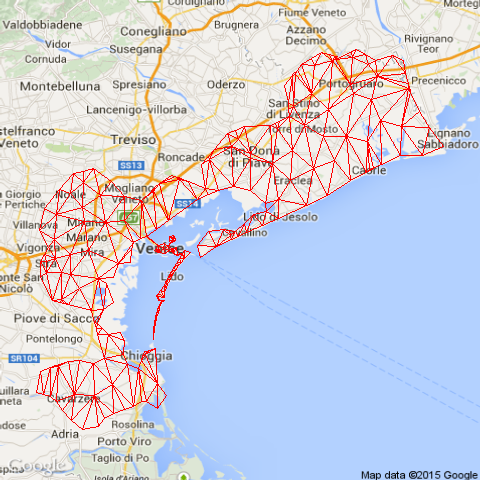
\includegraphics[width=0.46\textwidth]{Immagini/Ven_triang.png}   
   }
\subfigure[Zoom della laguna]
   {
   \label{fig:Ven_triang_zoom}
	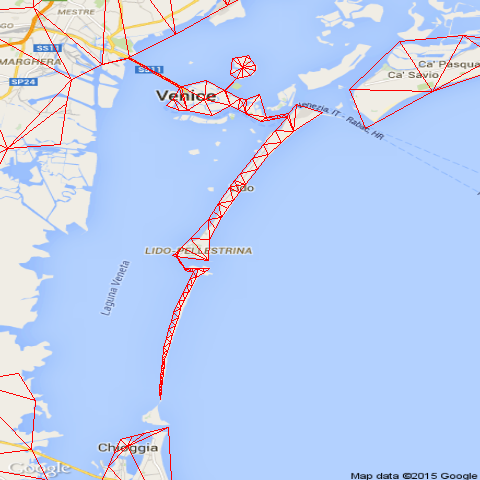
\includegraphics[width=0.46\textwidth]{Immagini/Ven_triangzoom.png}
   }
\caption{Triangolazione della provincia di Venezia}
\label{fig:Ven_triang}
\end{figure}

In conclusione, il dominio è descritto da 414 punti (41 con dati, 373 di frontiera o aggiunti dalla triangolazione) e da 475 triangoli. 

\section{Applicazione del modello senza covariate}

\subsection{Analisi preliminare e ricerca del miglior $\underline \lambda$}
Le basi in spazio scelte per l'applicazione del modello in questo caso sono gli elementi finiti lineari. Ad ognuno dei punti spaziali (interni o di frontiera) è associata una funzione di base, coerentemente con la triangolazione prodotta. Di conseguenza, si ha $N=414$ mentre il numero di punti con dati $n$ è minore ed è pari a 41.

In tempo, esattamente come nel caso del dominio a forma di C, sono state scelte come funzioni di base le B-splines cubiche. L'intervallo temporale per la descrizione del dominio è $[1997,2011]$, e i dati sono disponibili con cadenza annuale. Anche in questo caso assumiamo che il numero di basi sia pari al numero di istanti temporali a disposizione, quindi $M=m=15$.

Prima di calcolare i risultati dell'analisi occorre fissare i parametri $\lambda_S$ e $\lambda_T$. Il procedimento è perfettamente analogo a quello ricavato nel caso del dominio a forma di C, minimizzando la quantità $GCV(\underline \lambda)$ in (CITAZIONE NECESSARIA). In tabella sono disponibili i risultati.

\begin{table}[htbp]
\renewcommand{\arraystretch}{1.3}
\setlength{\tabcolsep}{2mm}
\centering
	\begin{tabular}{!{\vrule width 1.2pt}c!{\vrule width 1.2pt}c!{\vrule width 1.2pt}}
	\noalign{\hrule height 1.2pt}
	Intervalli per $\log_{10}\lambda_S$ e $\log_{10}\lambda_T$& Miglior valore											\\
	\noalign{\hrule height 1.2pt}
	$\log_{10}\lambda_S \in \{-5,-4,\ldots,+1\}$ 	& \multirow{2}{*}{$\underline \lambda = (10^{0},10^{-3})$} 			\\
	\cline{1-1}
	$\log_{10}\lambda_T \in \{-5,-4,\ldots,+1\}$		& 															\\	
	\noalign{\hrule height 1.2pt}
	$\log_{10}\lambda_S \in \{-1,-0.75,\ldots,+1\}$ 	& \multirow{2}{*}{$\underline \lambda = (10^{-0.5},10^{-3.25})$} 		\\
	\cline{1-1}
	$\log_{10}\lambda_T \in \{-4,-3.75,\ldots,-2\}$	& 															\\	
	\noalign{\hrule height 1.2pt}
	$\log_{10}\lambda_S \in \{-1,-0.875,\ldots,+0\}$ 	& \multirow{2}{*}{$\underline \lambda = (10^{-0.375}, 10^{-3.25})$}	\\
	\cline{1-1}
	$\log_{10}\lambda_T \in \{-3.75,-3.625,\ldots,-2.75\}$		& 										6		\\	
	\noalign{\hrule height 1.2pt}
	\end{tabular}
\caption{Analisi di $\mathrm{GCV}(\underline \lambda)$}
\label{tab:Ven}
\end{table}

\subsection{Risultati}
La produzione dei rifiuti è stata analizzata con $\underline \lambda = (10^{-0.375}, 10^{-3.25})$. In fig. \ref{fig:Ven_ris} sono riportati i risultati ottenuti nei 15 anni a disposizione. Questi grafici (grazie anche alla visualizzazione sulle mappe di Google Maps) permettono di sutdiare il profilo della funzione nei vari istanti temporali, e avere un'idea dell'evoluzione della produzione di rifiuti a livello geografico.

\begin{figure}[H]
\centering
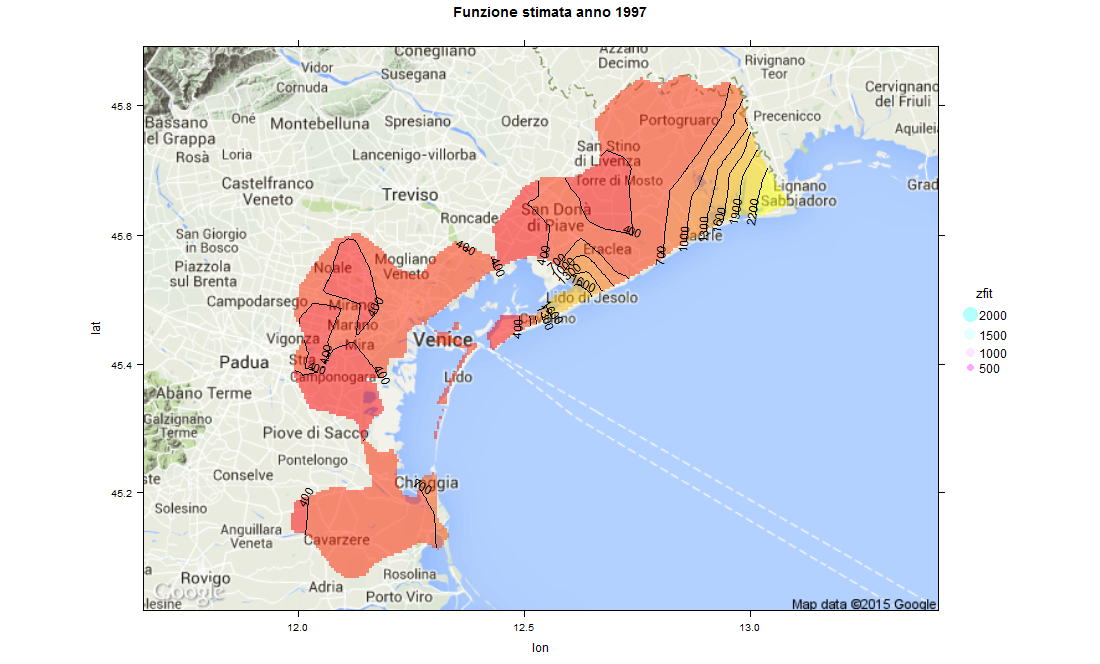
\includegraphics[trim=0cm 0cm 4cm 0cm,clip=true,width=0.32\textwidth]{Immagini/venezia_senza_covariate/Maps1997.png}
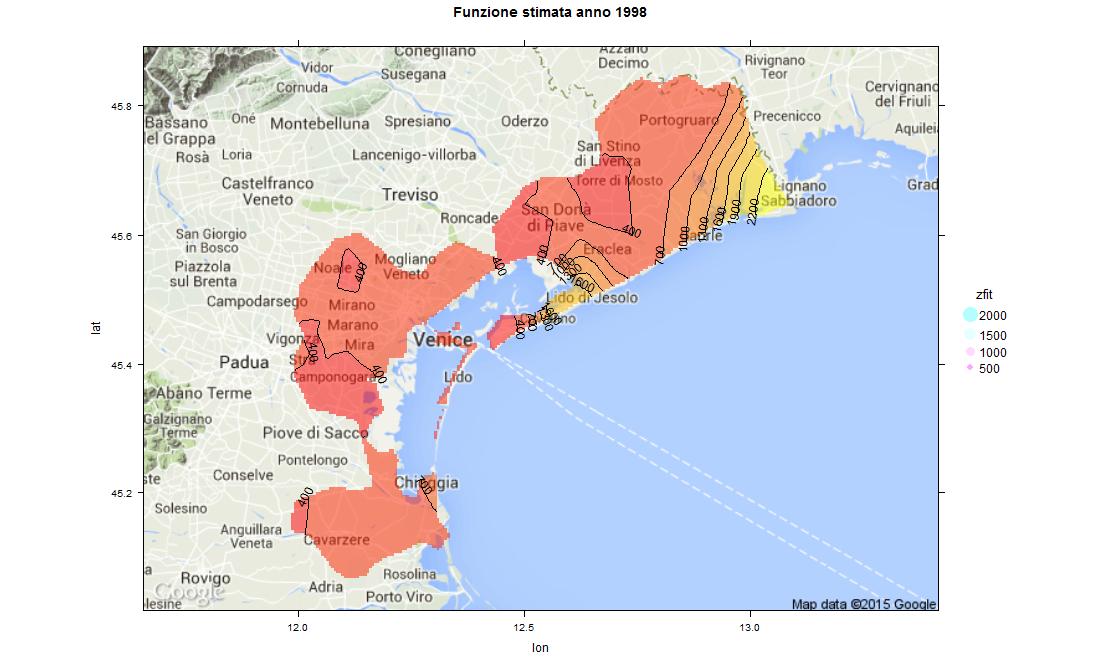
\includegraphics[trim=0cm 0cm 4cm 0cm,clip=true,width=0.32\textwidth]{Immagini/venezia_senza_covariate/Maps1998.png}
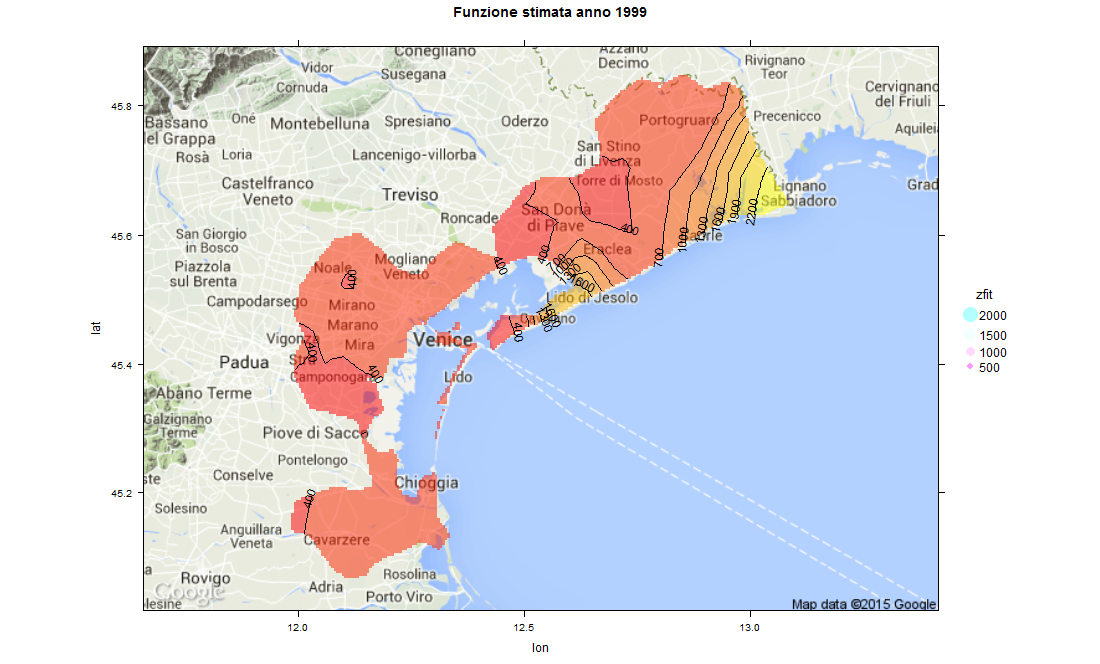
\includegraphics[trim=0cm 0cm 4cm 0cm,clip=true,width=0.32\textwidth]{Immagini/venezia_senza_covariate/Maps1999.png}
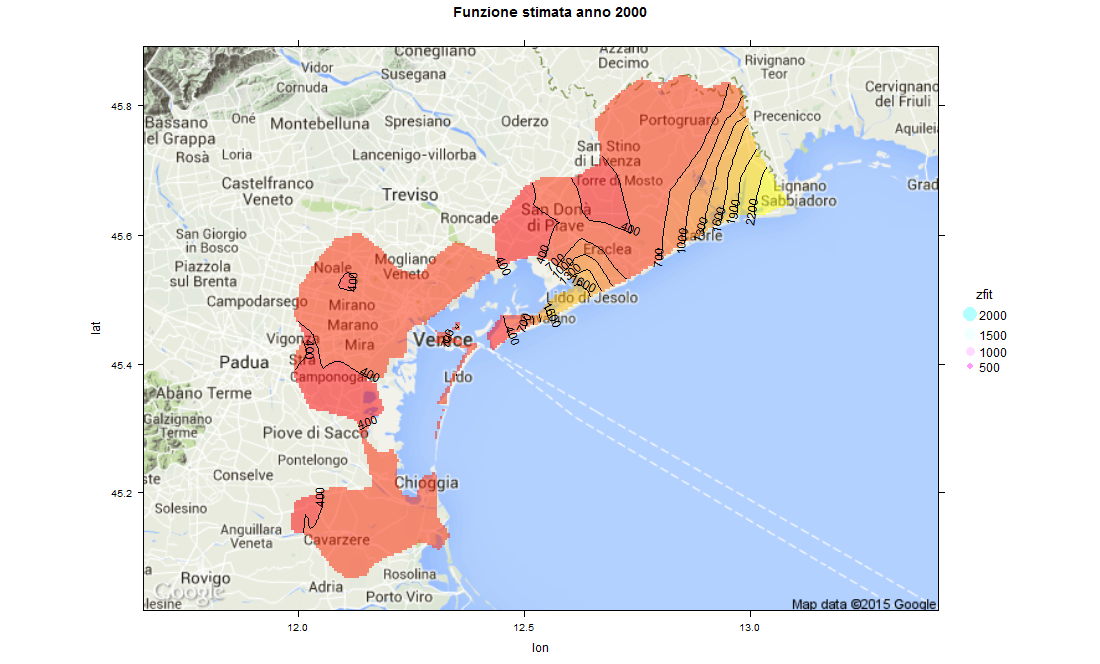
\includegraphics[trim=0cm 0cm 4cm 0cm,clip=true,width=0.32\textwidth]{Immagini/venezia_senza_covariate/Maps2000.png}
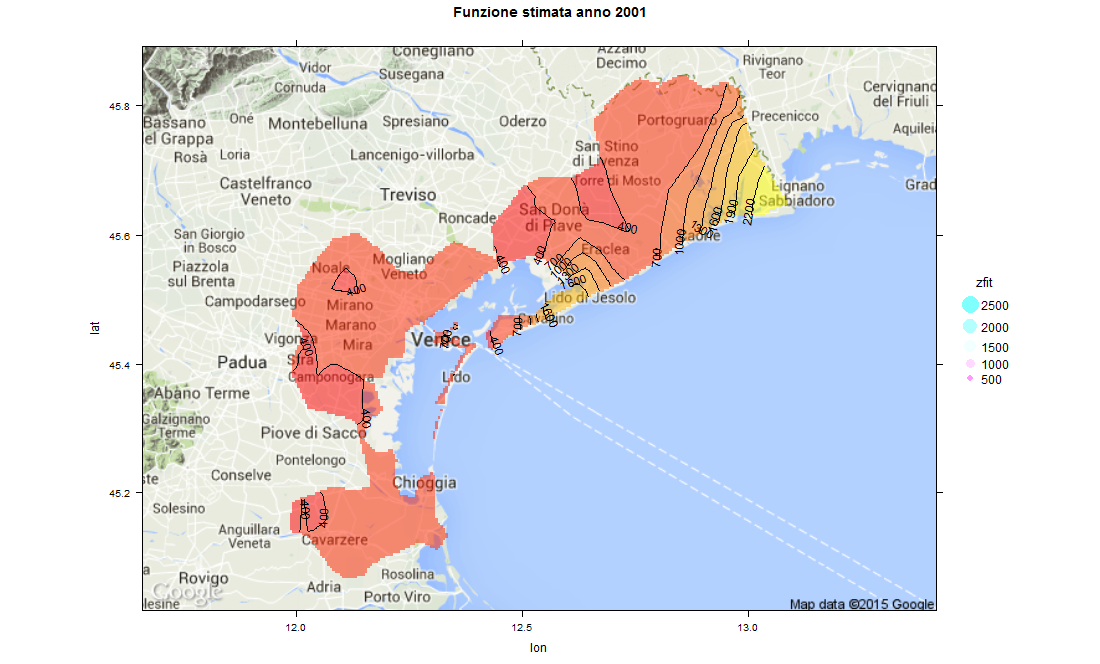
\includegraphics[trim=0cm 0cm 4cm 0cm,clip=true,width=0.32\textwidth]{Immagini/venezia_senza_covariate/Maps2001.png}
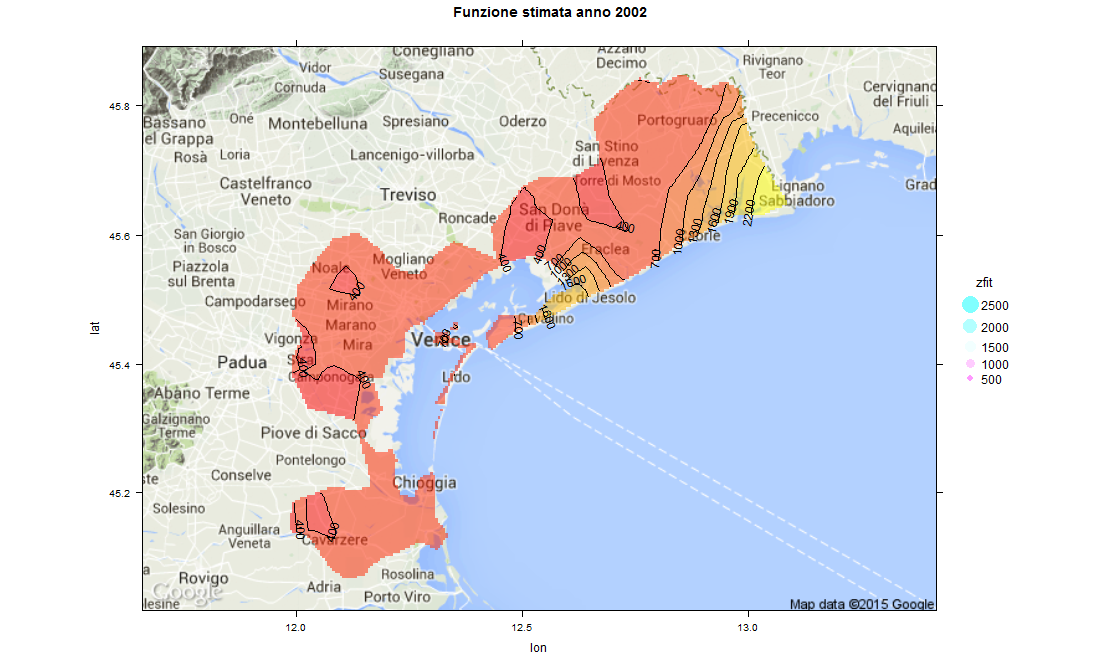
\includegraphics[trim=0cm 0cm 4cm 0cm,clip=true,width=0.32\textwidth]{Immagini/venezia_senza_covariate/Maps2002.png}
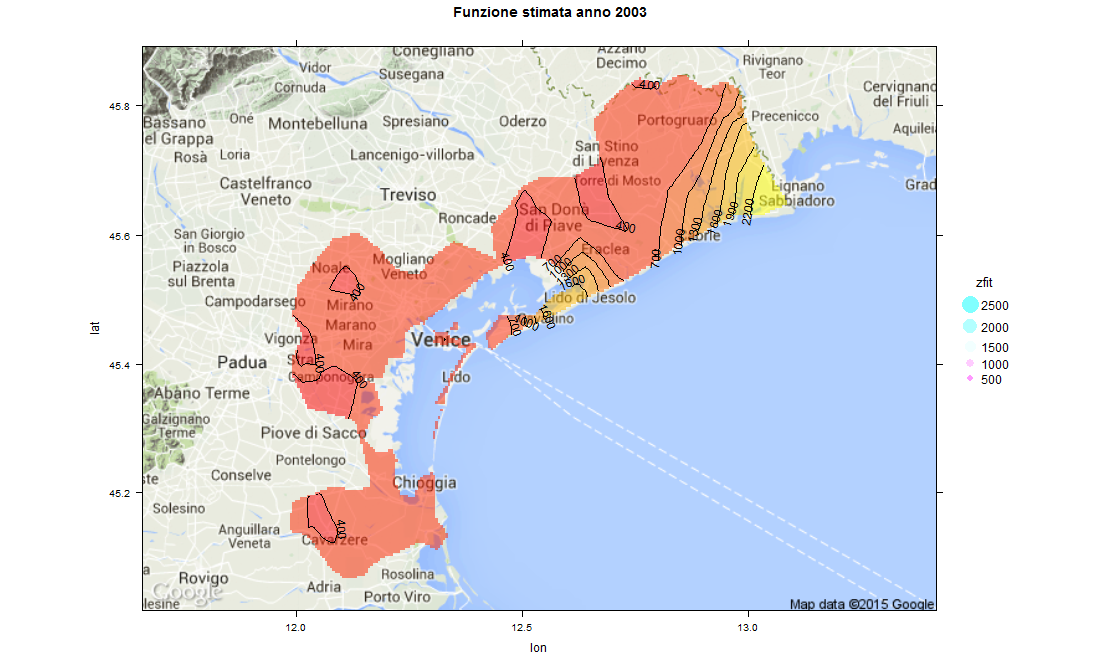
\includegraphics[trim=0cm 0cm 4cm 0cm,clip=true,width=0.32\textwidth]{Immagini/venezia_senza_covariate/Maps2003.png}
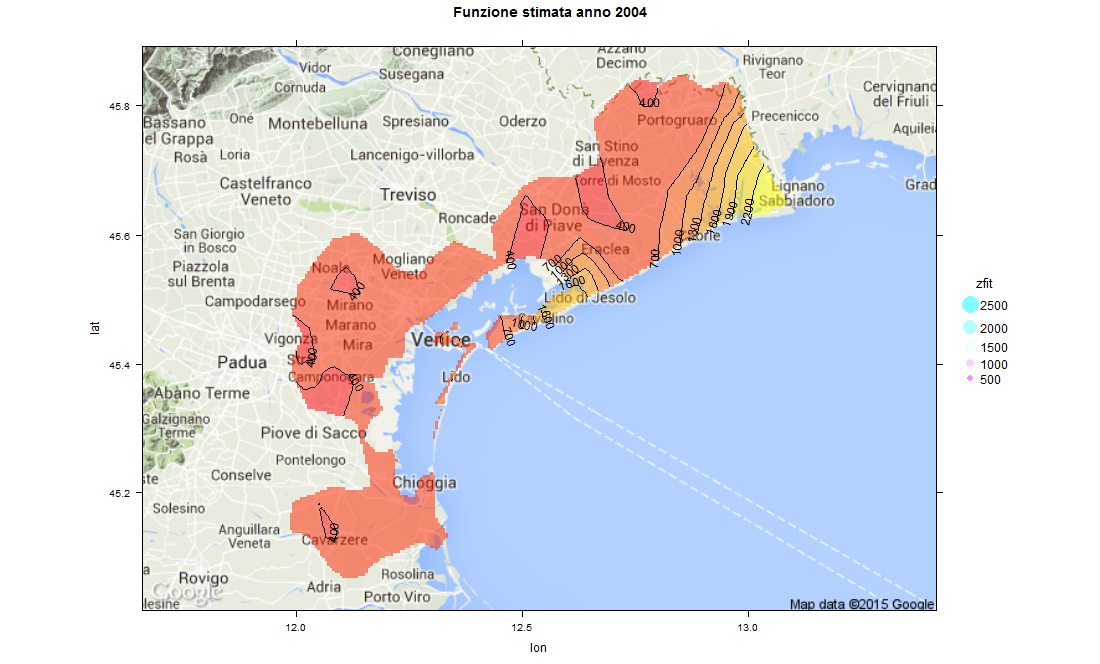
\includegraphics[trim=0cm 0cm 4cm 0cm,clip=true,width=0.32\textwidth]{Immagini/venezia_senza_covariate/Maps2004.png}
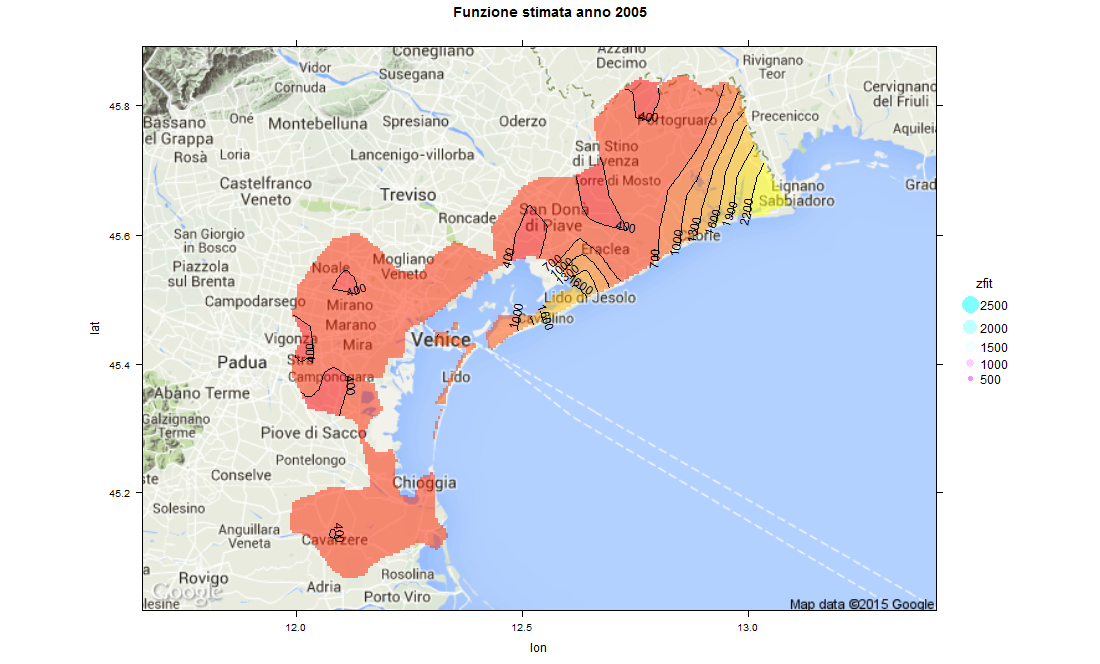
\includegraphics[trim=0cm 0cm 4cm 0cm,clip=true,width=0.32\textwidth]{Immagini/venezia_senza_covariate/Maps2005.png}
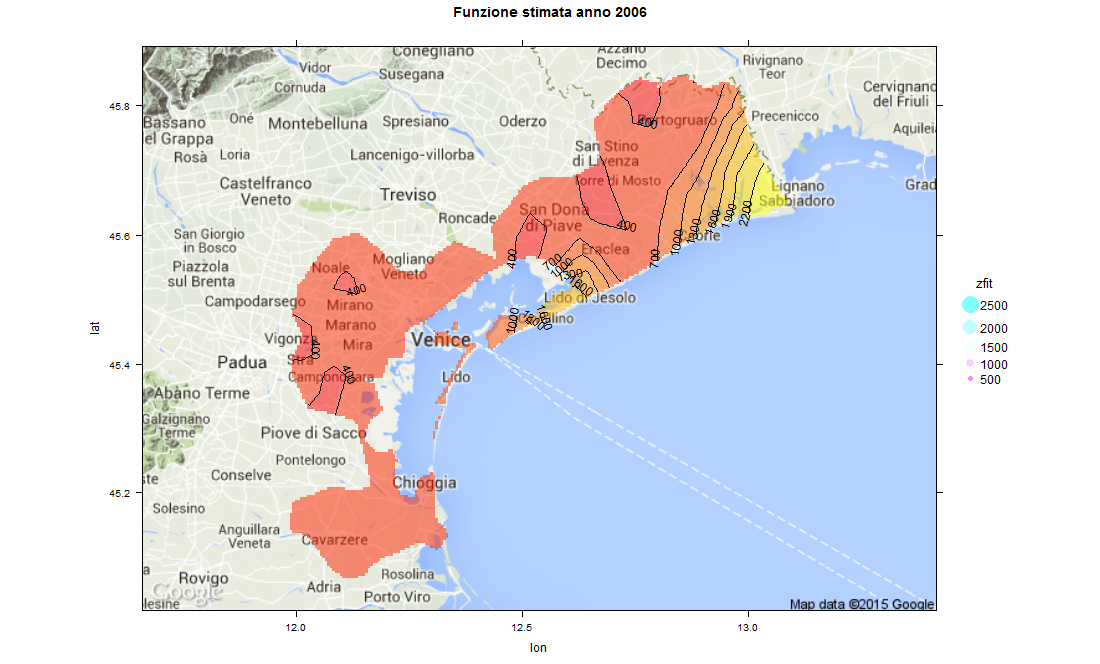
\includegraphics[trim=0cm 0cm 4cm 0cm,clip=true,width=0.32\textwidth]{Immagini/venezia_senza_covariate/Maps2006.png}
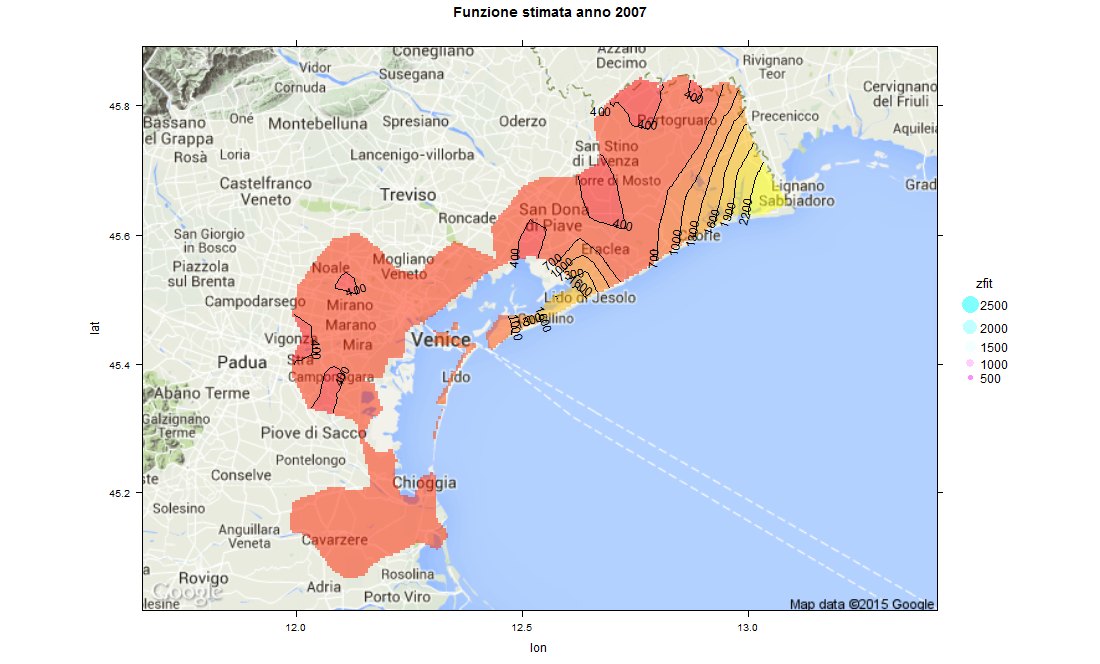
\includegraphics[trim=0cm 0cm 4cm 0cm,clip=true,width=0.32\textwidth]{Immagini/venezia_senza_covariate/Maps2007.png}
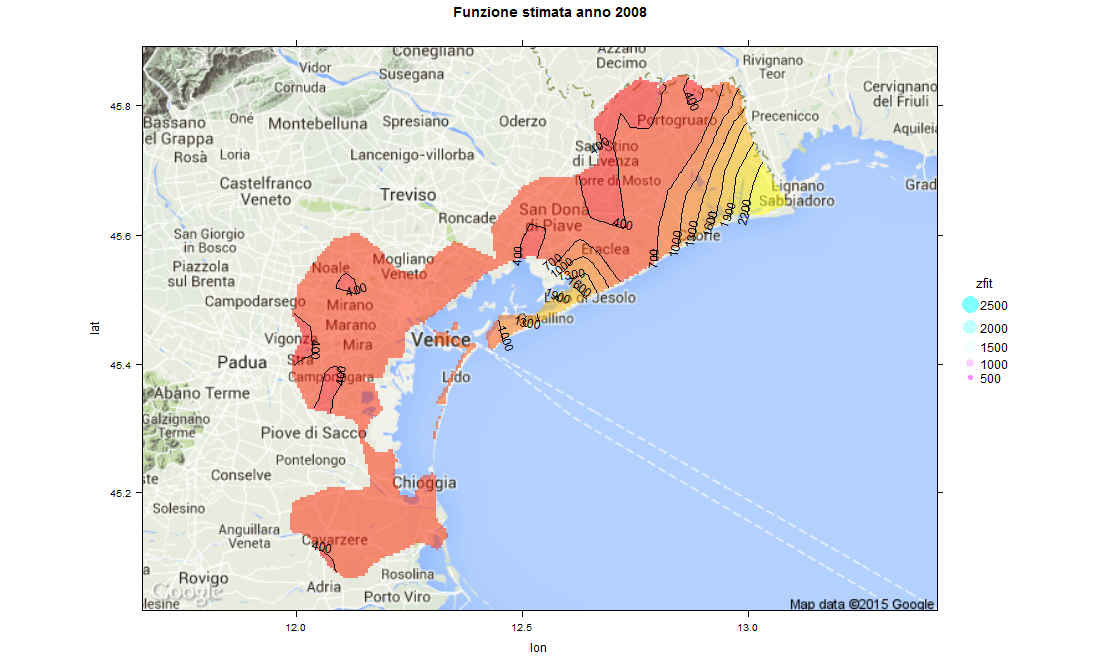
\includegraphics[trim=0cm 0cm 4cm 0cm,clip=true,width=0.32\textwidth]{Immagini/venezia_senza_covariate/Maps2008.png}
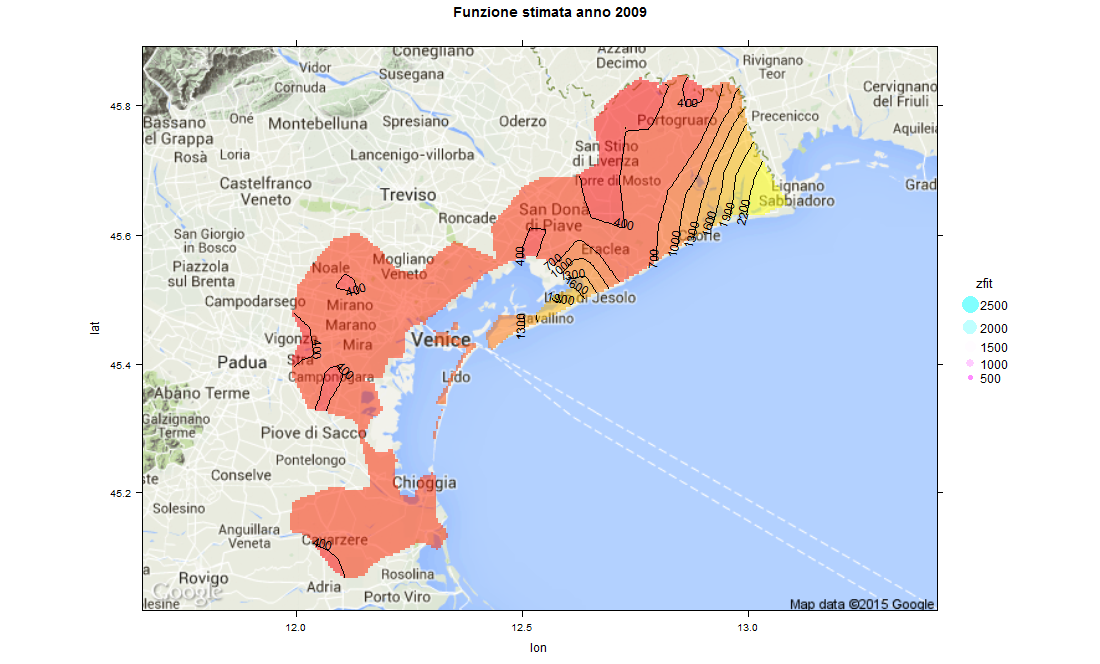
\includegraphics[trim=0cm 0cm 4cm 0cm,clip=true,width=0.32\textwidth]{Immagini/venezia_senza_covariate/Maps2009.png}
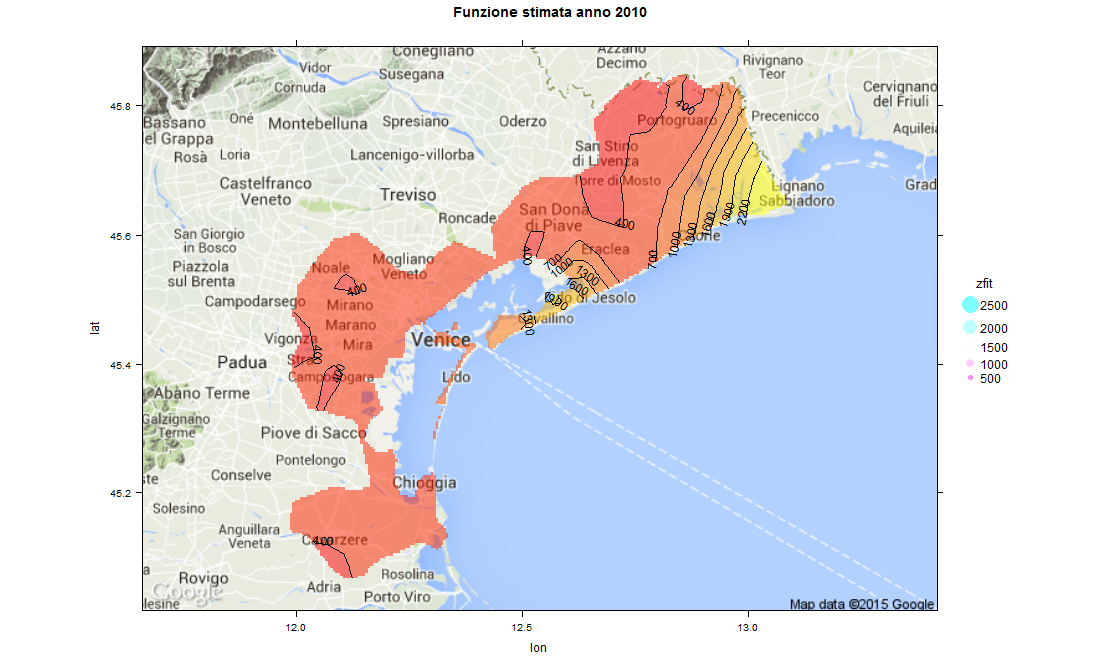
\includegraphics[trim=0cm 0cm 4cm 0cm,clip=true,width=0.32\textwidth]{Immagini/venezia_senza_covariate/Maps2010.png}
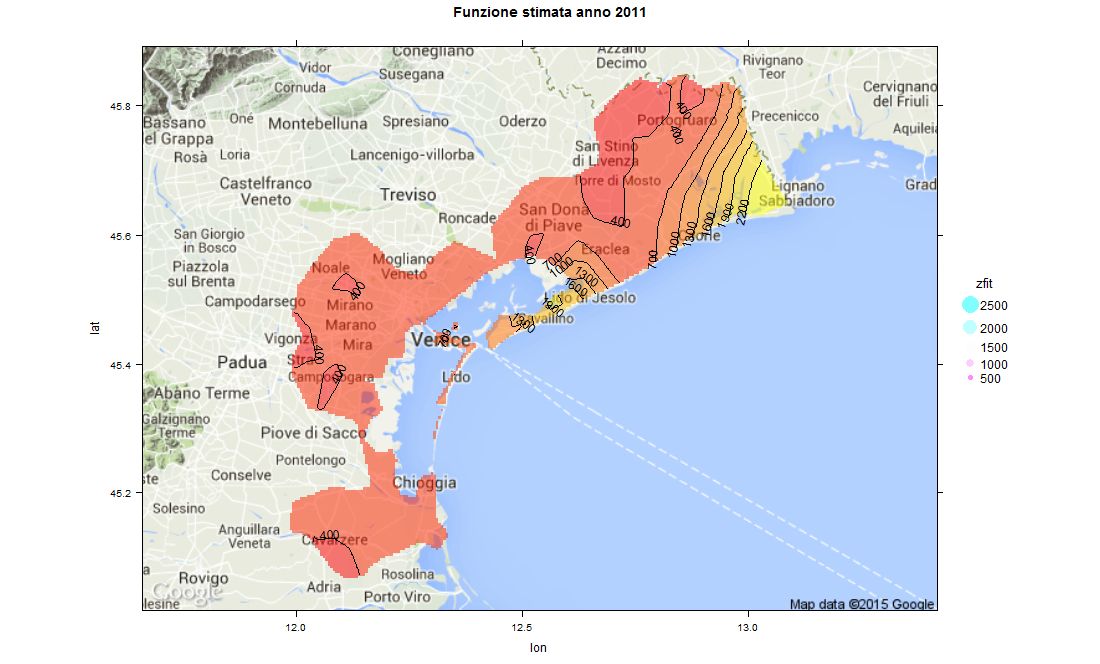
\includegraphics[trim=0cm 0cm 4cm 0cm,clip=true,width=0.32\textwidth]{Immagini/venezia_senza_covariate/Maps2011.png}
\caption{Estimated spatio-temporal field of the Venice waste data with the STSR method without covariates at fixed time instants: from year 1997 to year 2011.}
\label{fig:Ven_ris}
\end{figure}

Come si può notare dai grafici, ci sono due zone ad elevato valore di produzione dei rifiuti pro capite, corrispondenti a zone di elevato interesse turistico per le spiagge presenti. Nella parte ad est della provincia di Venezia, tra le altre, si hanno le località turistiche di Bibione (confinante con Lingano Sabbiadoro, che però è oltre il confine veneto) e Caorle. Scendendo verso sud-ovest si nota che anche Jesolo causa un innalzamento della funzione che descrive la risposta.

La produzione dei rifiuti è particolarmente alta in queste zone turistiche, e contrariamente a ciò che si poteva immaginare, molto di più di Venezia. Quindi già adesso possiamo immaginare che il turismo sarà rilevante nell'analisi della produzione di rifiuti, e la causa non sarà Venezia (dove la produzione non è eccessivamente diversa dagli altri comuni) ma le località balneari.

\begin{figure}[H]
\centering
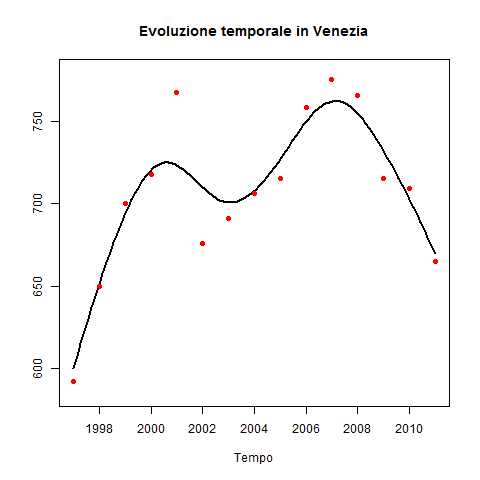
\includegraphics[width=0.32\textwidth]{Immagini/venezia_senza_covariate/Venezia.png}
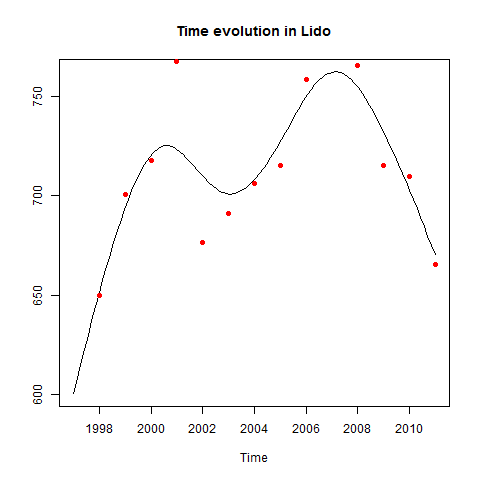
\includegraphics[width=0.32\textwidth]{Immagini/venezia_senza_covariate/Lido(A).png}
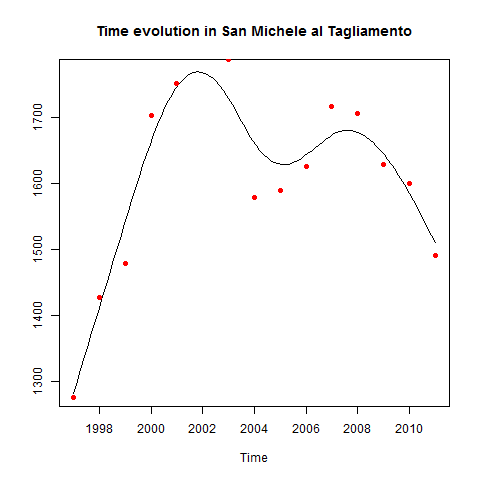
\includegraphics[width=0.32\textwidth]{Immagini/venezia_senza_covariate/SanMicheleTagliamento.png}
\caption{Estimated spatio-temporal field of the Venice waste data with the STSR method without covariates at three fixed spatial points: Venice, Lido and San Michele al Tagliamento.}
\label{fig:Ven_tempo}
\end{figure}

In fig. \ref{fig:venezia_tempo} Sono riportati gli sviluppi temporali stimati in alcuni comuni dati. In particolare sono stati scelti Venezia, Jesolo e Caorle). Si può notare come la funzione stimata spieghi bene l'andamento tracciato dai dati iniziali senza cadere nell'eccessiva interpolazione.

\section{Applicazione del modello con covariate}

\subsection{Analisi preliminare e ricerca del miglior $\underline \lambda$}
Le basi in spazio e in tempo sono esattamente le stesse del caso precedente. Prima di eseguire l'analisi, come al solito, occorre cercare buoni valori per $\underline \lambda$. Dalla tabella si possono seguire le iterazioni eseguite e il risultato finale.

\begin{table}[htbp]
\renewcommand{\arraystretch}{1.3}
\setlength{\tabcolsep}{2mm}
\centering
	\begin{tabular}{!{\vrule width 1.2pt}c!{\vrule width 1.2pt}c!{\vrule width 1.2pt}}
	\noalign{\hrule height 1.2pt}
	Intervalli per $\log_{10}\lambda_S$ e $\log_{10}\lambda_T$& Miglior valore											\\
	\noalign{\hrule height 1.2pt}
	$\log_{10}\lambda_S \in \{-5,-4,\ldots,+1\}$ 	& \multirow{2}{*}{$\underline \lambda = (10^{0},10^{-3})$} 			\\
	\cline{1-1}
	$\log_{10}\lambda_T \in \{-5,-4,\ldots,+1\}$		& 															\\	
	\noalign{\hrule height 1.2pt}
	$\log_{10}\lambda_S \in \{-1,-0.75,\ldots,+1\}$ 	& \multirow{2}{*}{$\underline \lambda = (10^{-0.5},10^{-3.25})$} 		\\
	\cline{1-1}
	$\log_{10}\lambda_T \in \{-4,-3.75,\ldots,-2\}$	& 															\\	
	\noalign{\hrule height 1.2pt}
	$\log_{10}\lambda_S \in \{-1,-0.875,\ldots,+0\}$ 	& \multirow{2}{*}{$\underline \lambda = (10^{-0.375}, 10^{-3.25})$}	\\
	\cline{1-1}
	$\log_{10}\lambda_T \in \{-3.75,-3.625,\ldots,-2.75\}$		& 										6		\\	
	\noalign{\hrule height 1.2pt}
	\end{tabular}
\caption{Analisi di $\mathrm{GCV}(\underline \lambda)$}
\label{tab:Vencovar}
\end{table}

\subsection{Risultati}
Le analisi sono state eseguite con $\underline \lambda = (10^{-0.375}, 10^{-3.25})$. Come si può notare dai grafici in fig. \ref{fig:Vencovar_ris}, dove è riportata la stima della funzione $f(\underline p,t)$ in ogni punti senza l'aggiunta della parte spiegata dalla covariata, nelle zone dove la produzione di rifiuti è massima si hanno ora i valori più bassi.

\begin{figure}[H]
\centering
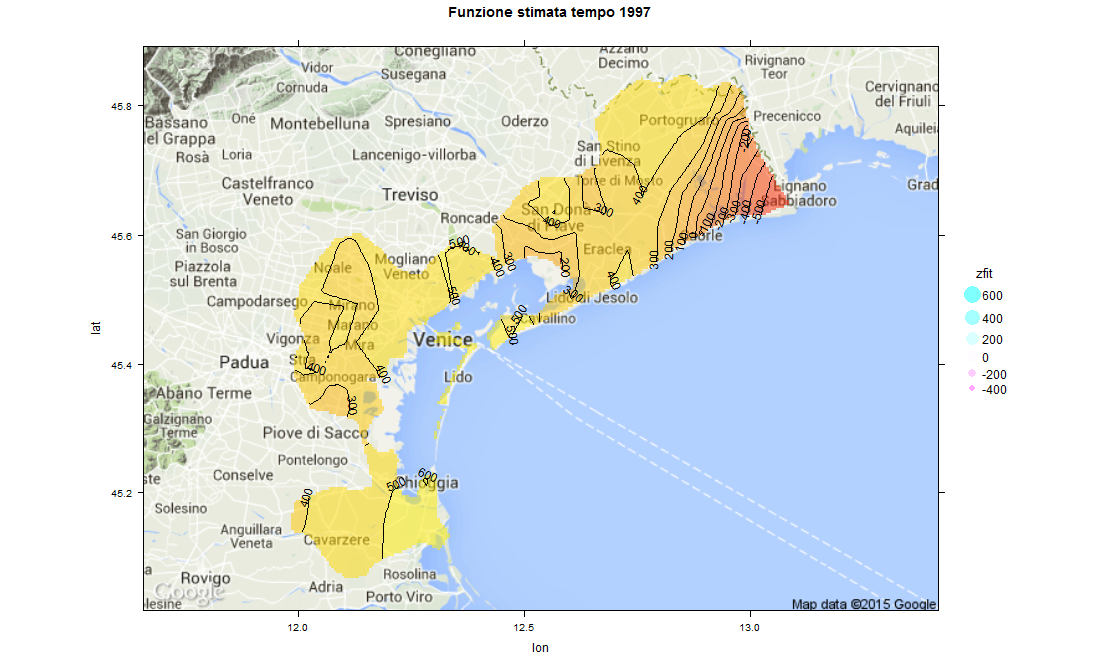
\includegraphics[trim=0cm 0cm 4cm 0cm,clip=true,width=0.32\textwidth]{Immagini/venezia_con_covariate/Maps1997.png}
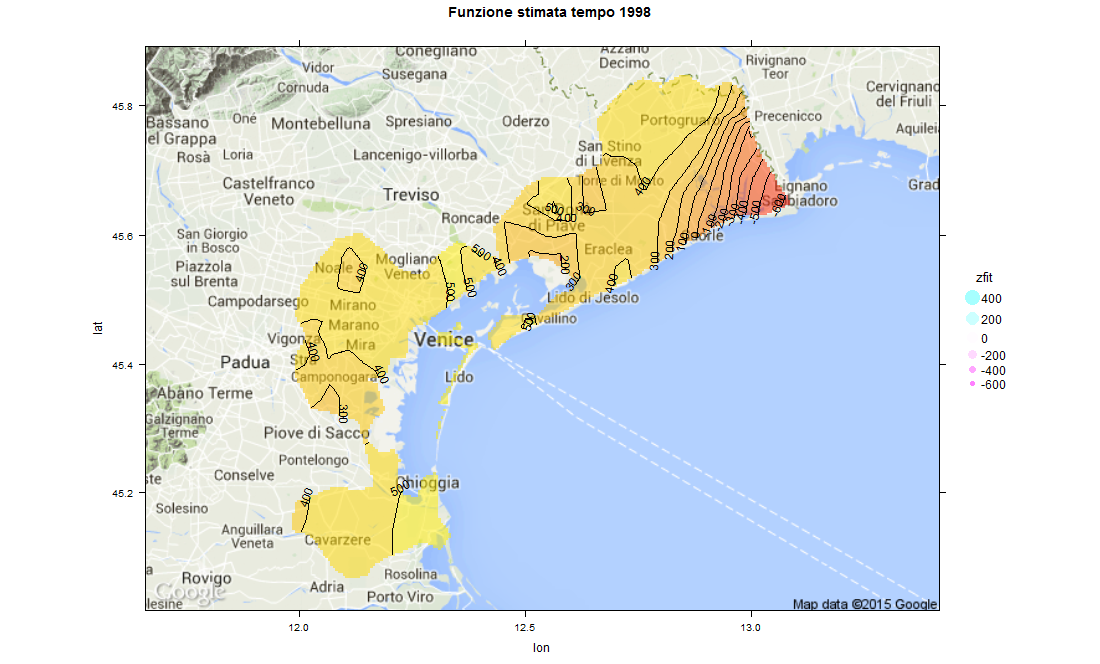
\includegraphics[trim=0cm 0cm 4cm 0cm,clip=true,width=0.32\textwidth]{Immagini/venezia_con_covariate/Maps1998.png}
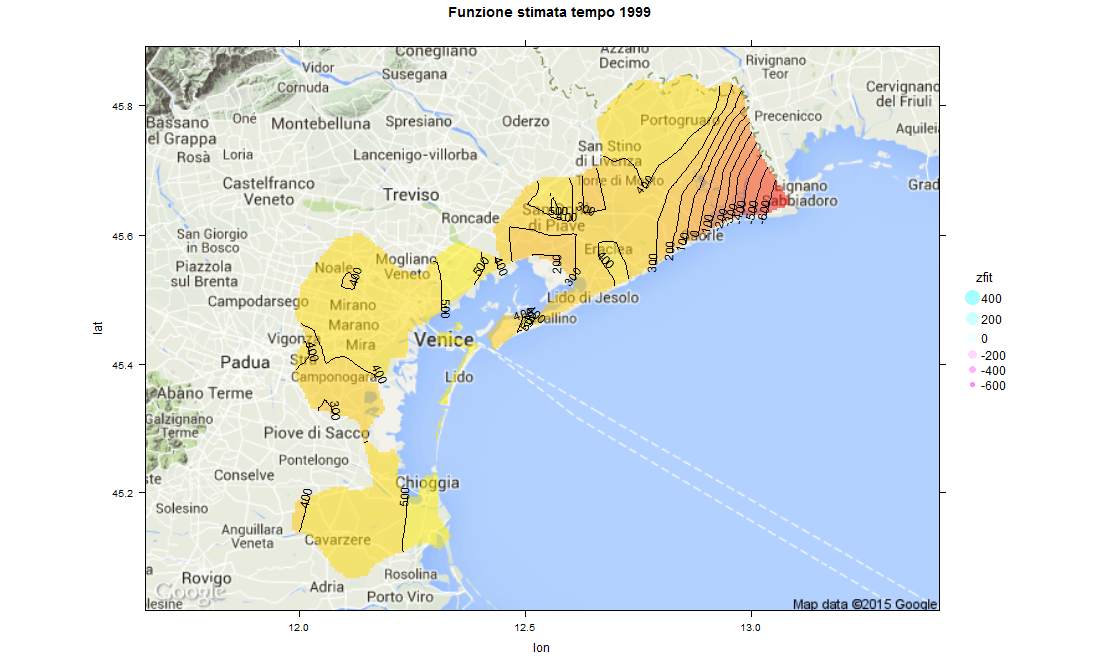
\includegraphics[trim=0cm 0cm 4cm 0cm,clip=true,width=0.32\textwidth]{Immagini/venezia_con_covariate/Maps1999.png}
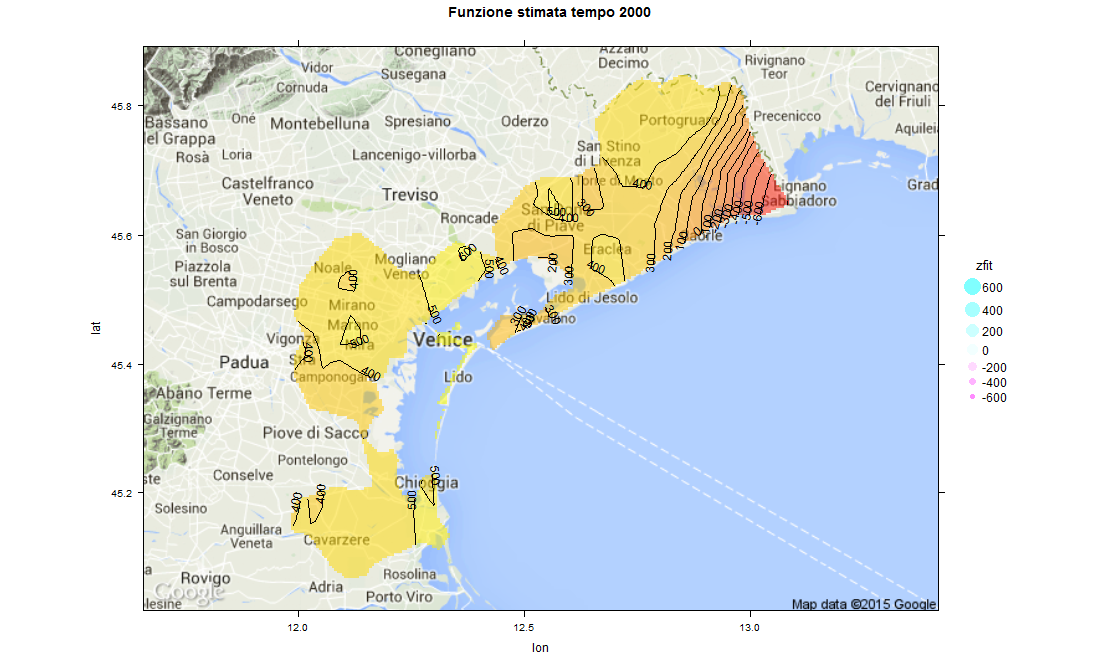
\includegraphics[trim=0cm 0cm 4cm 0cm,clip=true,width=0.32\textwidth]{Immagini/venezia_con_covariate/Maps2000.png}
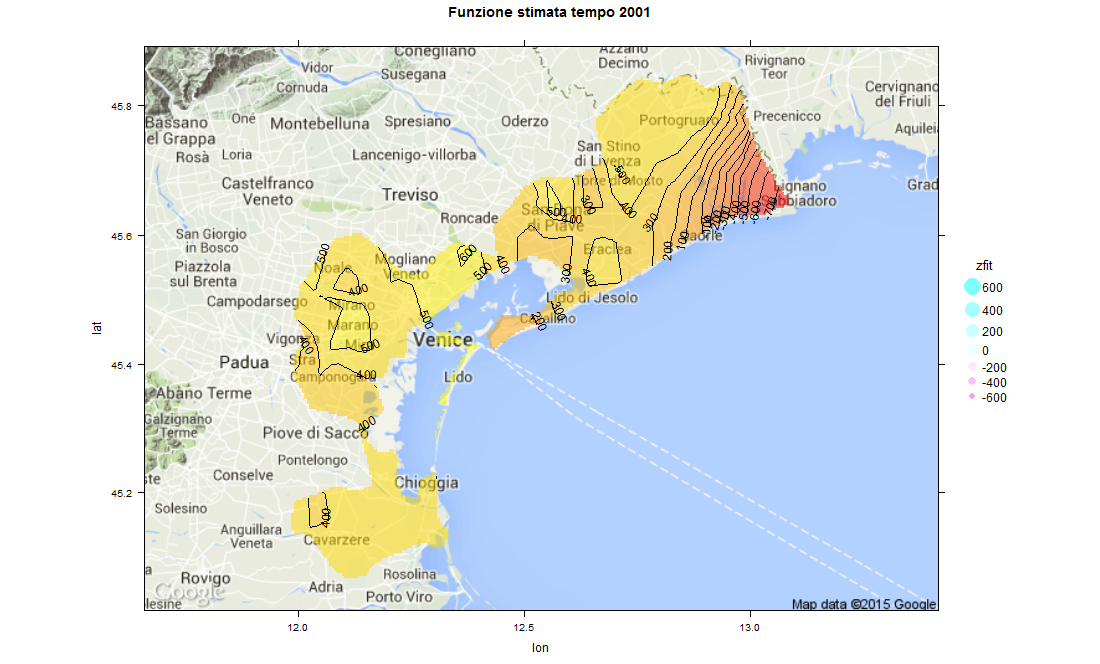
\includegraphics[trim=0cm 0cm 4cm 0cm,clip=true,width=0.32\textwidth]{Immagini/venezia_con_covariate/Maps2001.png}
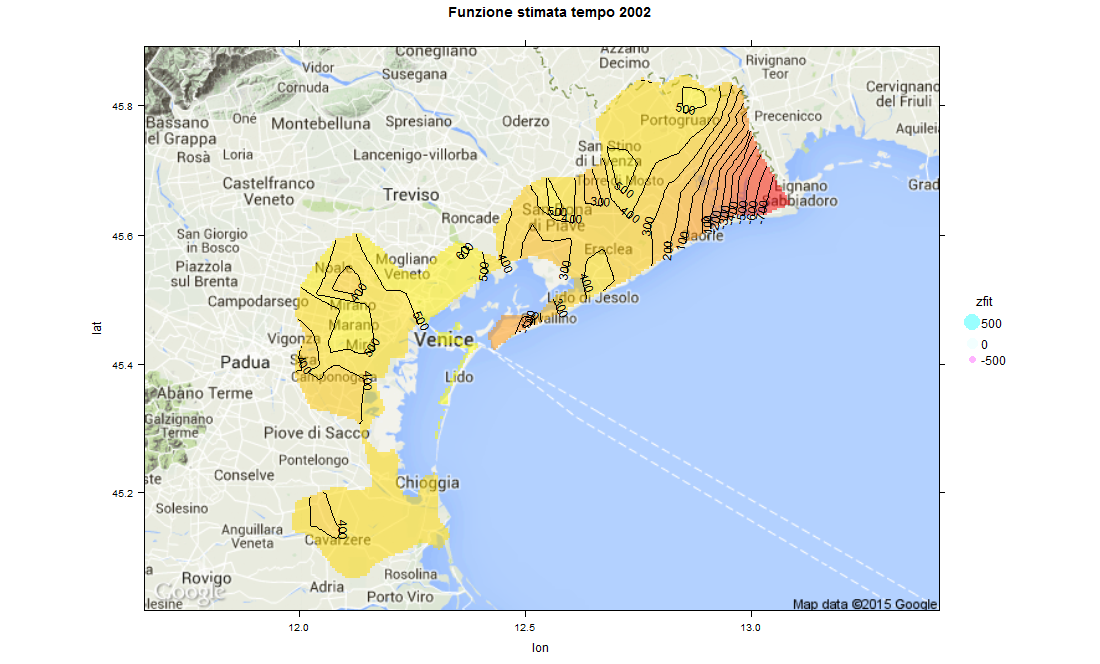
\includegraphics[trim=0cm 0cm 4cm 0cm,clip=true,width=0.32\textwidth]{Immagini/venezia_con_covariate/Maps2002.png}
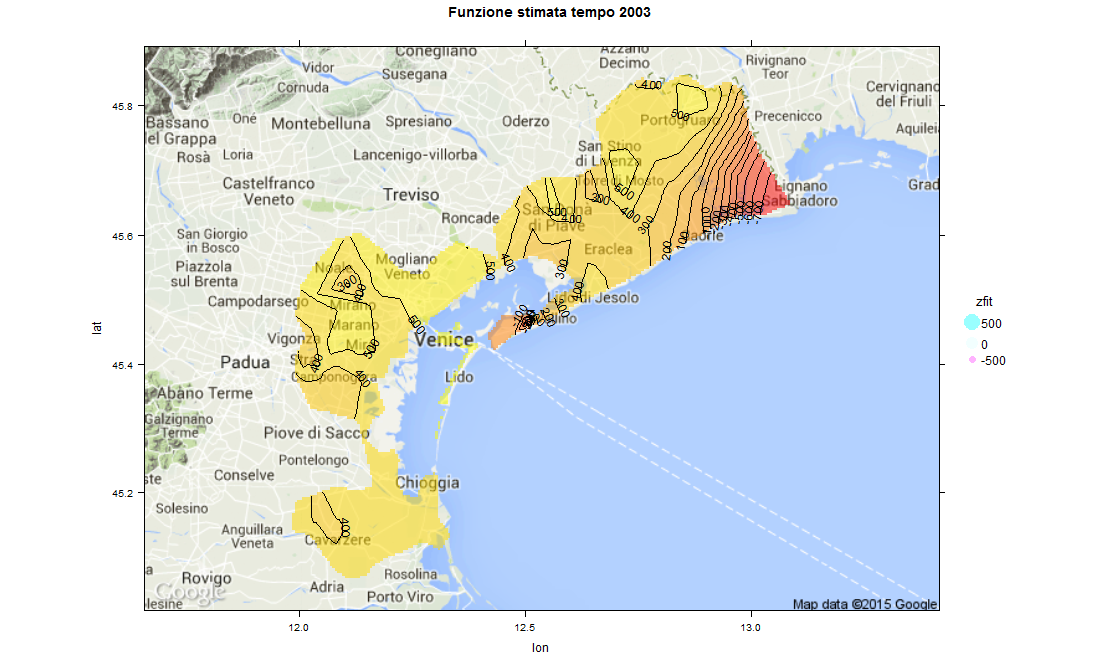
\includegraphics[trim=0cm 0cm 4cm 0cm,clip=true,width=0.32\textwidth]{Immagini/venezia_con_covariate/Maps2003.png}
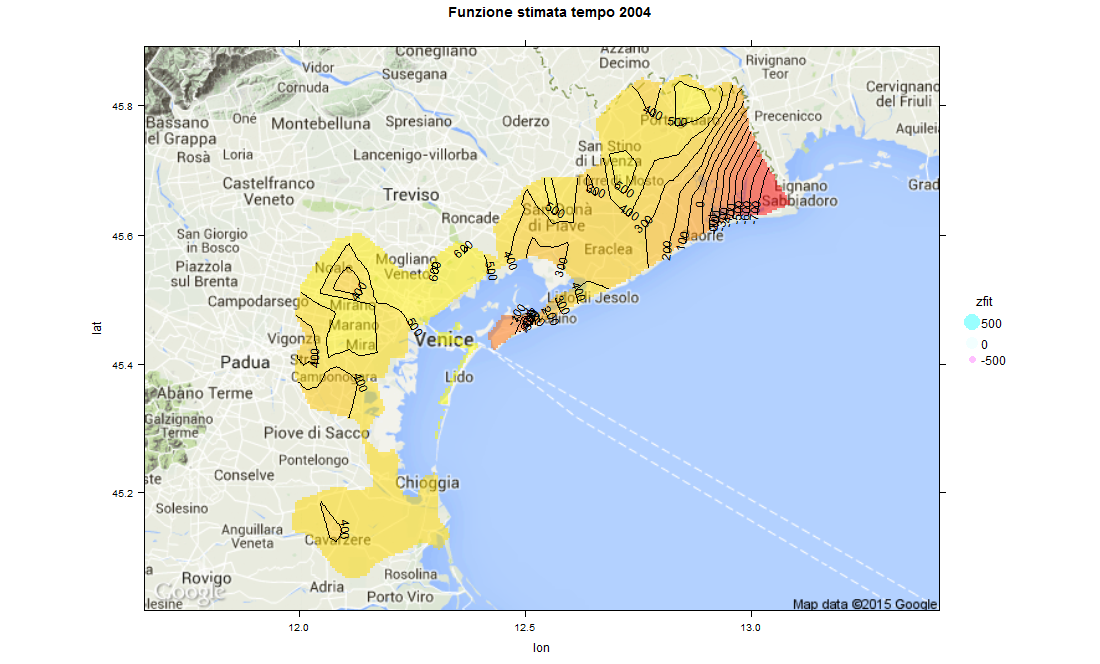
\includegraphics[trim=0cm 0cm 4cm 0cm,clip=true,width=0.32\textwidth]{Immagini/venezia_con_covariate/Maps2004.png}
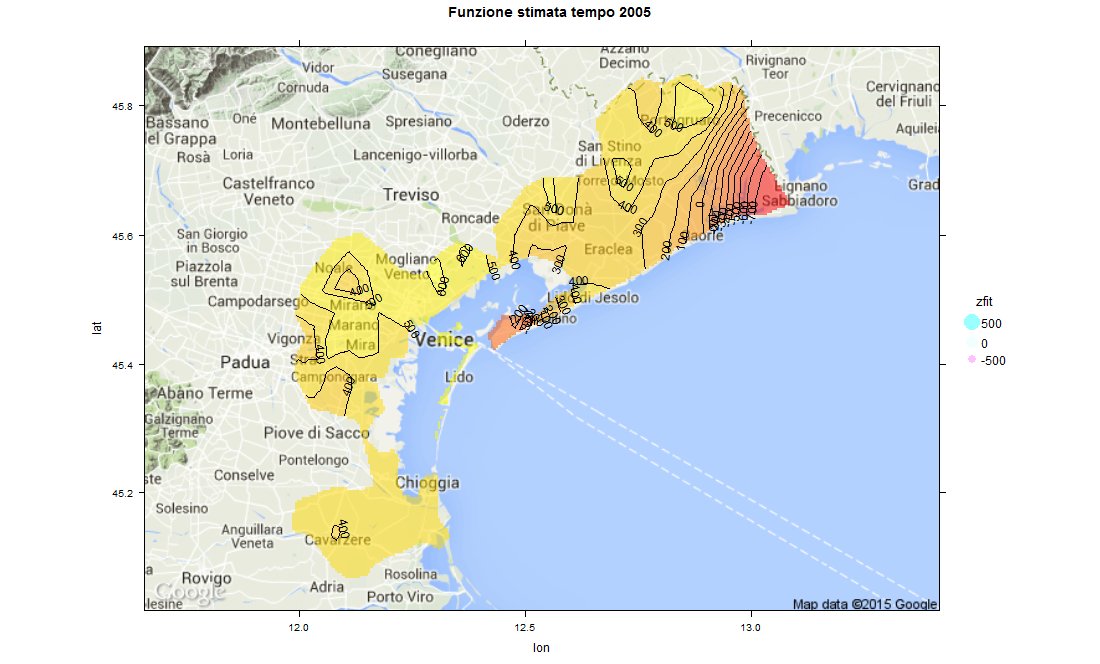
\includegraphics[trim=0cm 0cm 4cm 0cm,clip=true,width=0.32\textwidth]{Immagini/venezia_con_covariate/Maps2005.png}
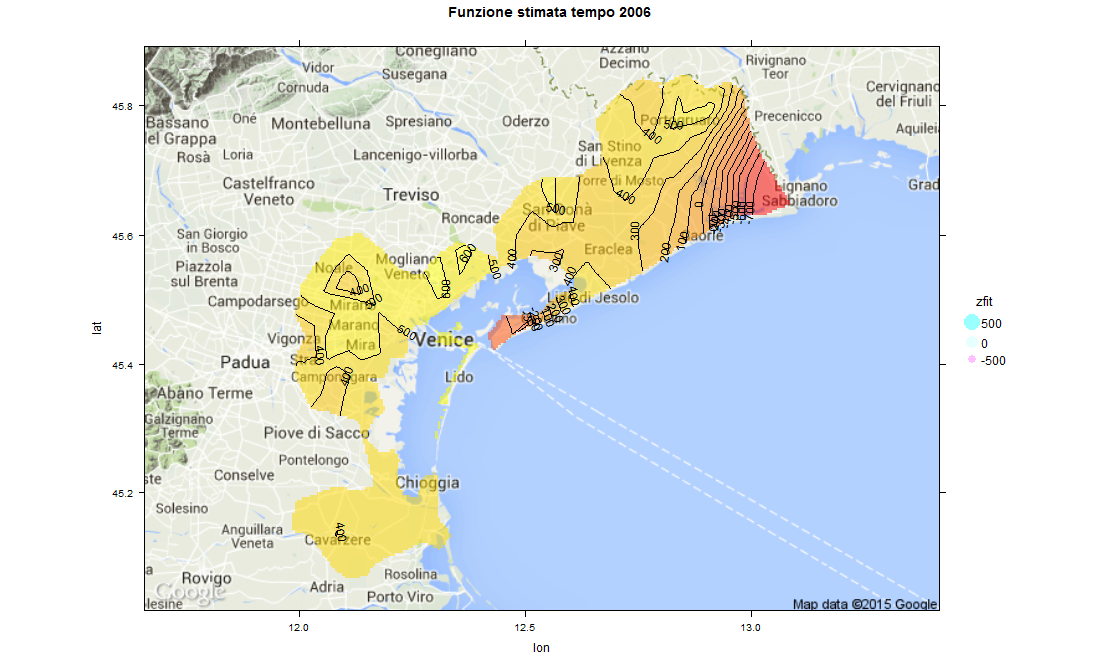
\includegraphics[trim=0cm 0cm 4cm 0cm,clip=true,width=0.32\textwidth]{Immagini/venezia_con_covariate/Maps2006.png}
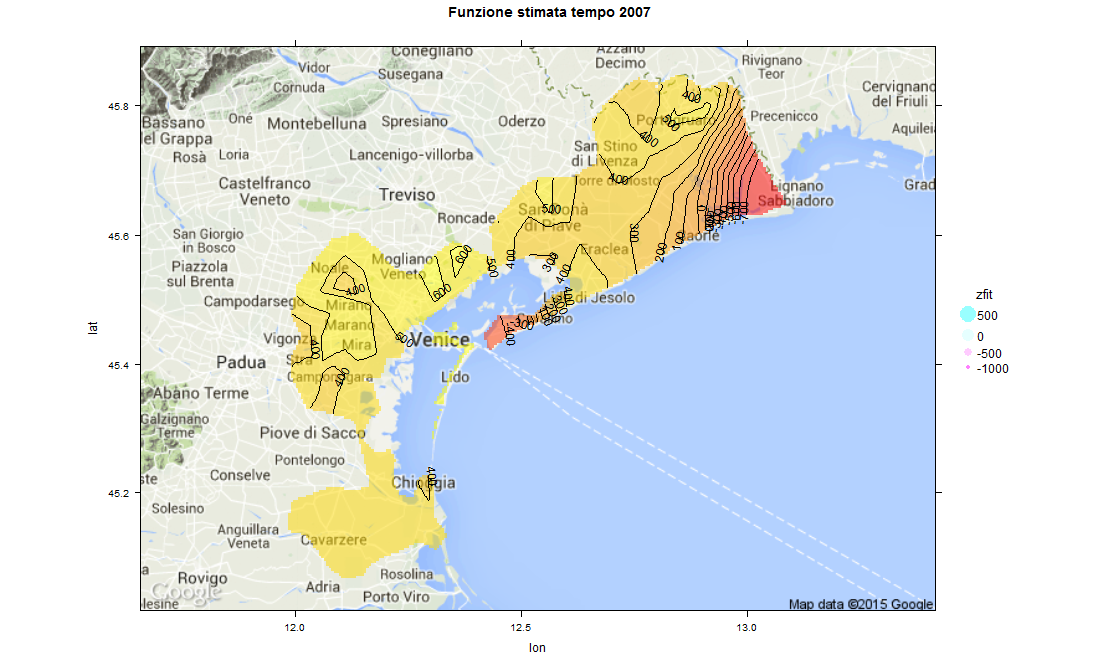
\includegraphics[trim=0cm 0cm 4cm 0cm,clip=true,width=0.32\textwidth]{Immagini/venezia_con_covariate/Maps2007.png}
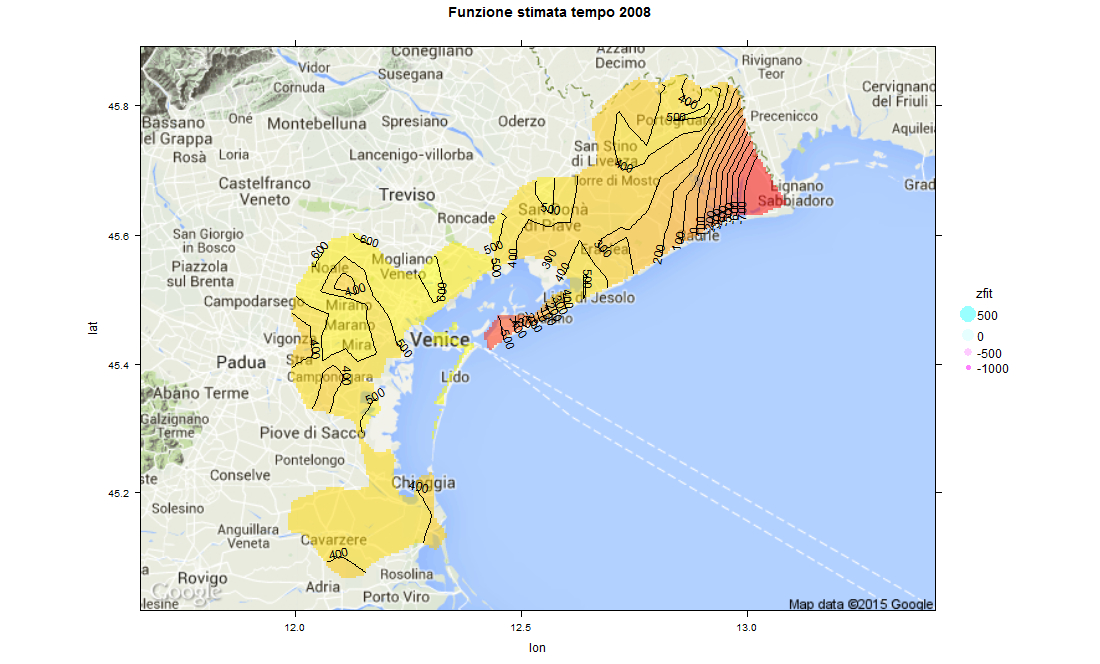
\includegraphics[trim=0cm 0cm 4cm 0cm,clip=true,width=0.32\textwidth]{Immagini/venezia_con_covariate/Maps2008.png}
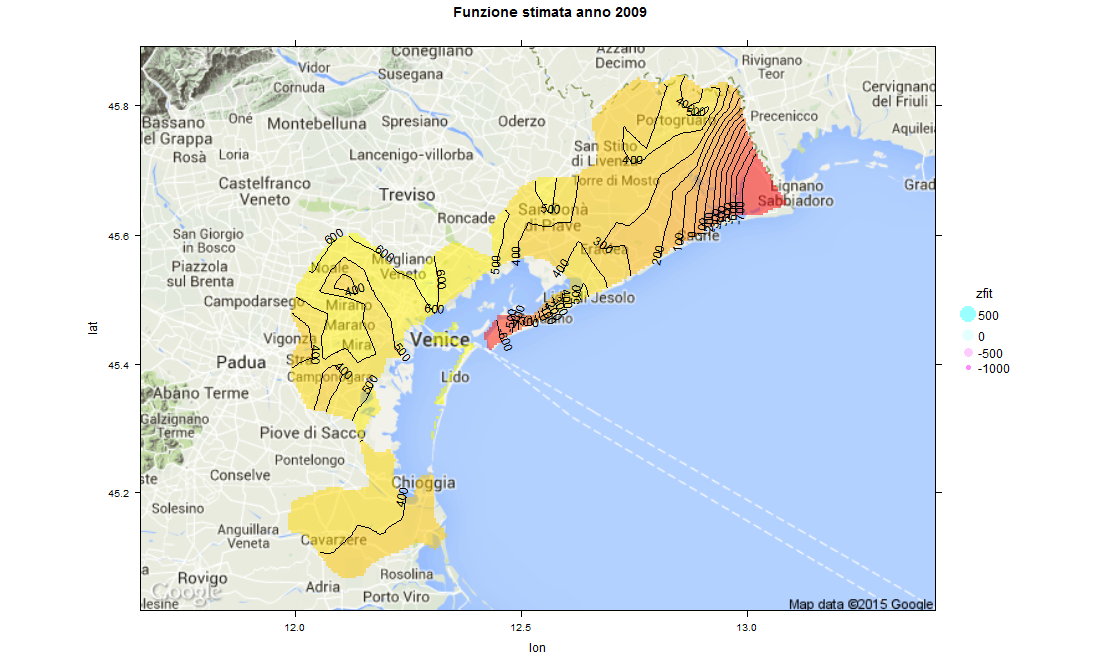
\includegraphics[trim=0cm 0cm 4cm 0cm,clip=true,width=0.32\textwidth]{Immagini/venezia_con_covariate/Maps2009.png}
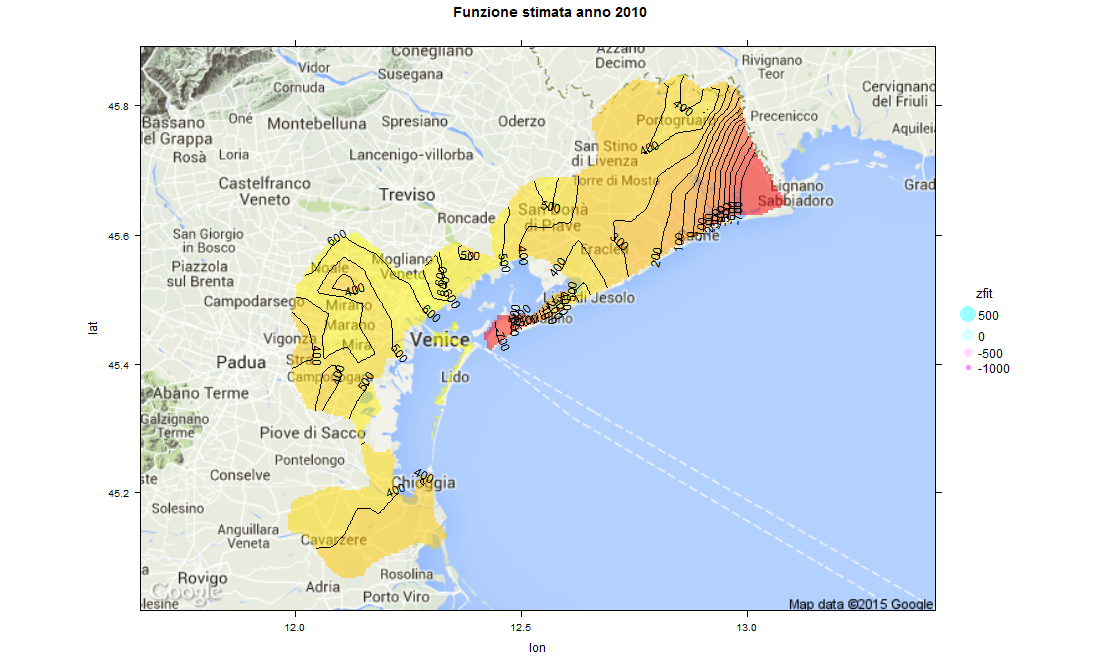
\includegraphics[trim=0cm 0cm 4cm 0cm,clip=true,width=0.32\textwidth]{Immagini/venezia_con_covariate/Maps2010.png}
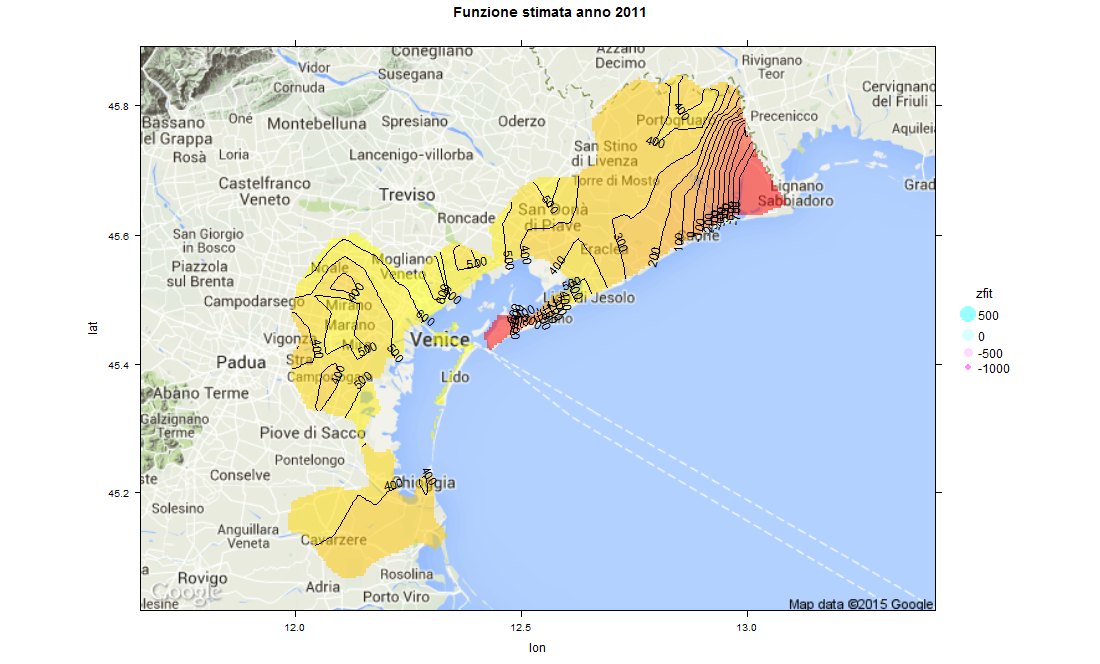
\includegraphics[trim=0cm 0cm 4cm 0cm,clip=true,width=0.32\textwidth]{Immagini/venezia_con_covariate/Maps2011.png}
\caption{Estimated spatio-temporal field of the Venice waste data with the STSR method without covariates at fixed time instants: from year 1997 to year 2011.}
\label{fig:Vencovar_ris}
\end{figure}

\begin{figure}[H]
\centering
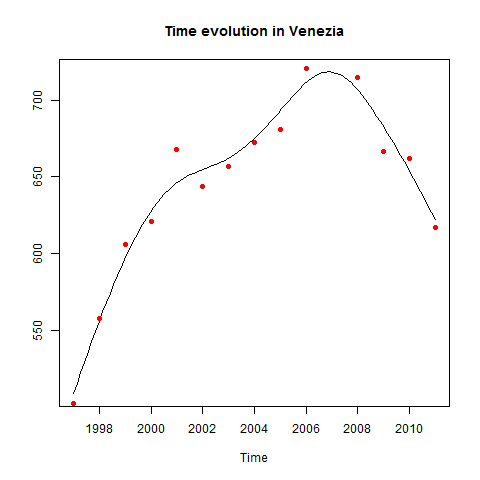
\includegraphics[width=0.32\textwidth]{Immagini/venezia_con_covariate/Venezia.png}
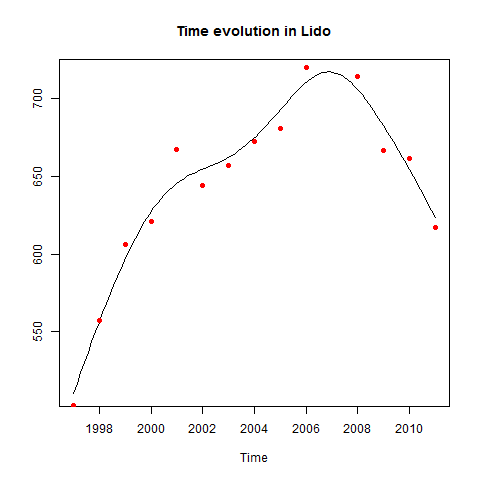
\includegraphics[width=0.32\textwidth]{Immagini/venezia_con_covariate/Lido(A).png}
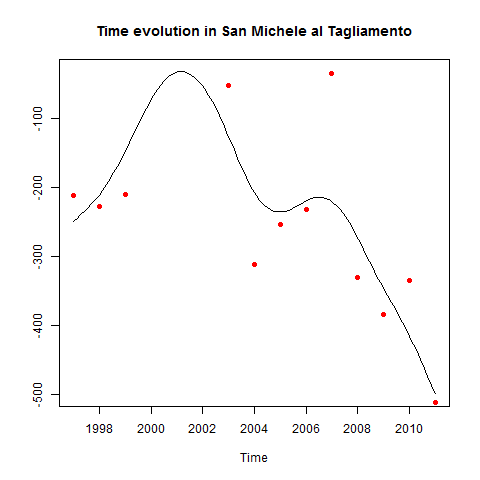
\includegraphics[width=0.32\textwidth]{Immagini/venezia_con_covariate/SanMicheleTagliamento.png}
\caption{Estimated spatio-temporal field of the Venice waste data with the STSR method without covariates at three fixed spatial points: Venice, Lido and San Michele al Tagliamento.}
\label{fig:Vencovar_tempo}
\end{figure}

In fig. \ref{fig:venezia_tempo} Sono riportati gli sviluppi temporali stimati in alcuni comuni dati. In particolare sono stati scelti Venezia, Jesolo e Caorle). Si può notare come la funzione stimata spieghi bene l'andamento tracciato dai dati iniziali senza cadere nell'eccessiva interpolazione.













\end{document}